\documentclass[1p]{elsarticle_modified}
%\bibliographystyle{elsarticle-num}

%\usepackage[colorlinks]{hyperref}
%\usepackage{abbrmath_seonhwa} %\Abb, \Ascr, \Acal ,\Abf, \Afrak
\usepackage{amsfonts}
\usepackage{amssymb}
\usepackage{amsmath}
\usepackage{amsthm}
\usepackage{scalefnt}
\usepackage{amsbsy}
\usepackage{kotex}
\usepackage{caption}
\usepackage{subfig}
\usepackage{color}
\usepackage{graphicx}
\usepackage{xcolor} %% white, black, red, green, blue, cyan, magenta, yellow
\usepackage{float}
\usepackage{setspace}
\usepackage{hyperref}

\usepackage{tikz}
\usetikzlibrary{arrows}

\usepackage{multirow}
\usepackage{array} % fixed length table
\usepackage{hhline}

%%%%%%%%%%%%%%%%%%%%%
\makeatletter
\renewcommand*\env@matrix[1][\arraystretch]{%
	\edef\arraystretch{#1}%
	\hskip -\arraycolsep
	\let\@ifnextchar\new@ifnextchar
	\array{*\c@MaxMatrixCols c}}
\makeatother %https://tex.stackexchange.com/questions/14071/how-can-i-increase-the-line-spacing-in-a-matrix
%%%%%%%%%%%%%%%

\usepackage[normalem]{ulem}

\newcommand{\msout}[1]{\ifmmode\text{\sout{\ensuremath{#1}}}\else\sout{#1}\fi}
%SOURCE: \msout is \stkout macro in https://tex.stackexchange.com/questions/20609/strikeout-in-math-mode

\newcommand{\cancel}[1]{
	\ifmmode
	{\color{red}\msout{#1}}
	\else
	{\color{red}\sout{#1}}
	\fi
}

\newcommand{\add}[1]{
	{\color{blue}\uwave{#1}}
}

\newcommand{\replace}[2]{
	\ifmmode
	{\color{red}\msout{#1}}{\color{blue}\uwave{#2}}
	\else
	{\color{red}\sout{#1}}{\color{blue}\uwave{#2}}
	\fi
}

\newcommand{\Sol}{\mathcal{S}} %segment
\newcommand{\D}{D} %diagram
\newcommand{\A}{\mathcal{A}} %arc


%%%%%%%%%%%%%%%%%%%%%%%%%%%%%5 test

\def\sl{\operatorname{\textup{SL}}(2,\Cbb)}
\def\psl{\operatorname{\textup{PSL}}(2,\Cbb)}
\def\quan{\mkern 1mu \triangleright \mkern 1mu}

\theoremstyle{definition}
\newtheorem{thm}{Theorem}[section]
\newtheorem{prop}[thm]{Proposition}
\newtheorem{lem}[thm]{Lemma}
\newtheorem{ques}[thm]{Question}
\newtheorem{cor}[thm]{Corollary}
\newtheorem{defn}[thm]{Definition}
\newtheorem{exam}[thm]{Example}
\newtheorem{rmk}[thm]{Remark}
\newtheorem{alg}[thm]{Algorithm}

\newcommand{\I}{\sqrt{-1}}
\begin{document}

%\begin{frontmatter}
%
%\title{Boundary parabolic representations of knots up to 8 crossings}
%
%%% Group authors per affiliation:
%\author{Yunhi Cho} 
%\address{Department of Mathematics, University of Seoul, Seoul, Korea}
%\ead{yhcho@uos.ac.kr}
%
%
%\author{Seonhwa Kim} %\fnref{s_kim}}
%\address{Center for Geometry and Physics, Institute for Basic Science, Pohang, 37673, Korea}
%\ead{ryeona17@ibs.re.kr}
%
%\author{Hyuk Kim}
%\address{Department of Mathematical Sciences, Seoul National University, Seoul 08826, Korea}
%\ead{hyukkim@snu.ac.kr}
%
%\author{Seokbeom Yoon}
%\address{Department of Mathematical Sciences, Seoul National University, Seoul, 08826,  Korea}
%\ead{sbyoon15@snu.ac.kr}
%
%\begin{abstract}
%We find all boundary parabolic representation of knots up to 8 crossings.
%
%\end{abstract}
%\begin{keyword}
%    \MSC[2010] 57M25 
%\end{keyword}
%
%\end{frontmatter}

%\linenumbers
%\tableofcontents
%
\newcommand\colored[1]{\textcolor{white}{\rule[-0.35ex]{0.8em}{1.4ex}}\kern-0.8em\color{red} #1}%
%\newcommand\colored[1]{\textcolor{white}{ #1}\kern-2.17ex	\textcolor{white}{ #1}\kern-1.81ex	\textcolor{white}{ #1}\kern-2.15ex\color{red}#1	}

{\Large $\underline{12a_{0966}~(K12a_{0966})}$}

\setlength{\tabcolsep}{10pt}
\renewcommand{\arraystretch}{1.6}
\vspace{1cm}\begin{tabular}{m{100pt}>{\centering\arraybackslash}m{274pt}}
\multirow{5}{120pt}{
	\centering
	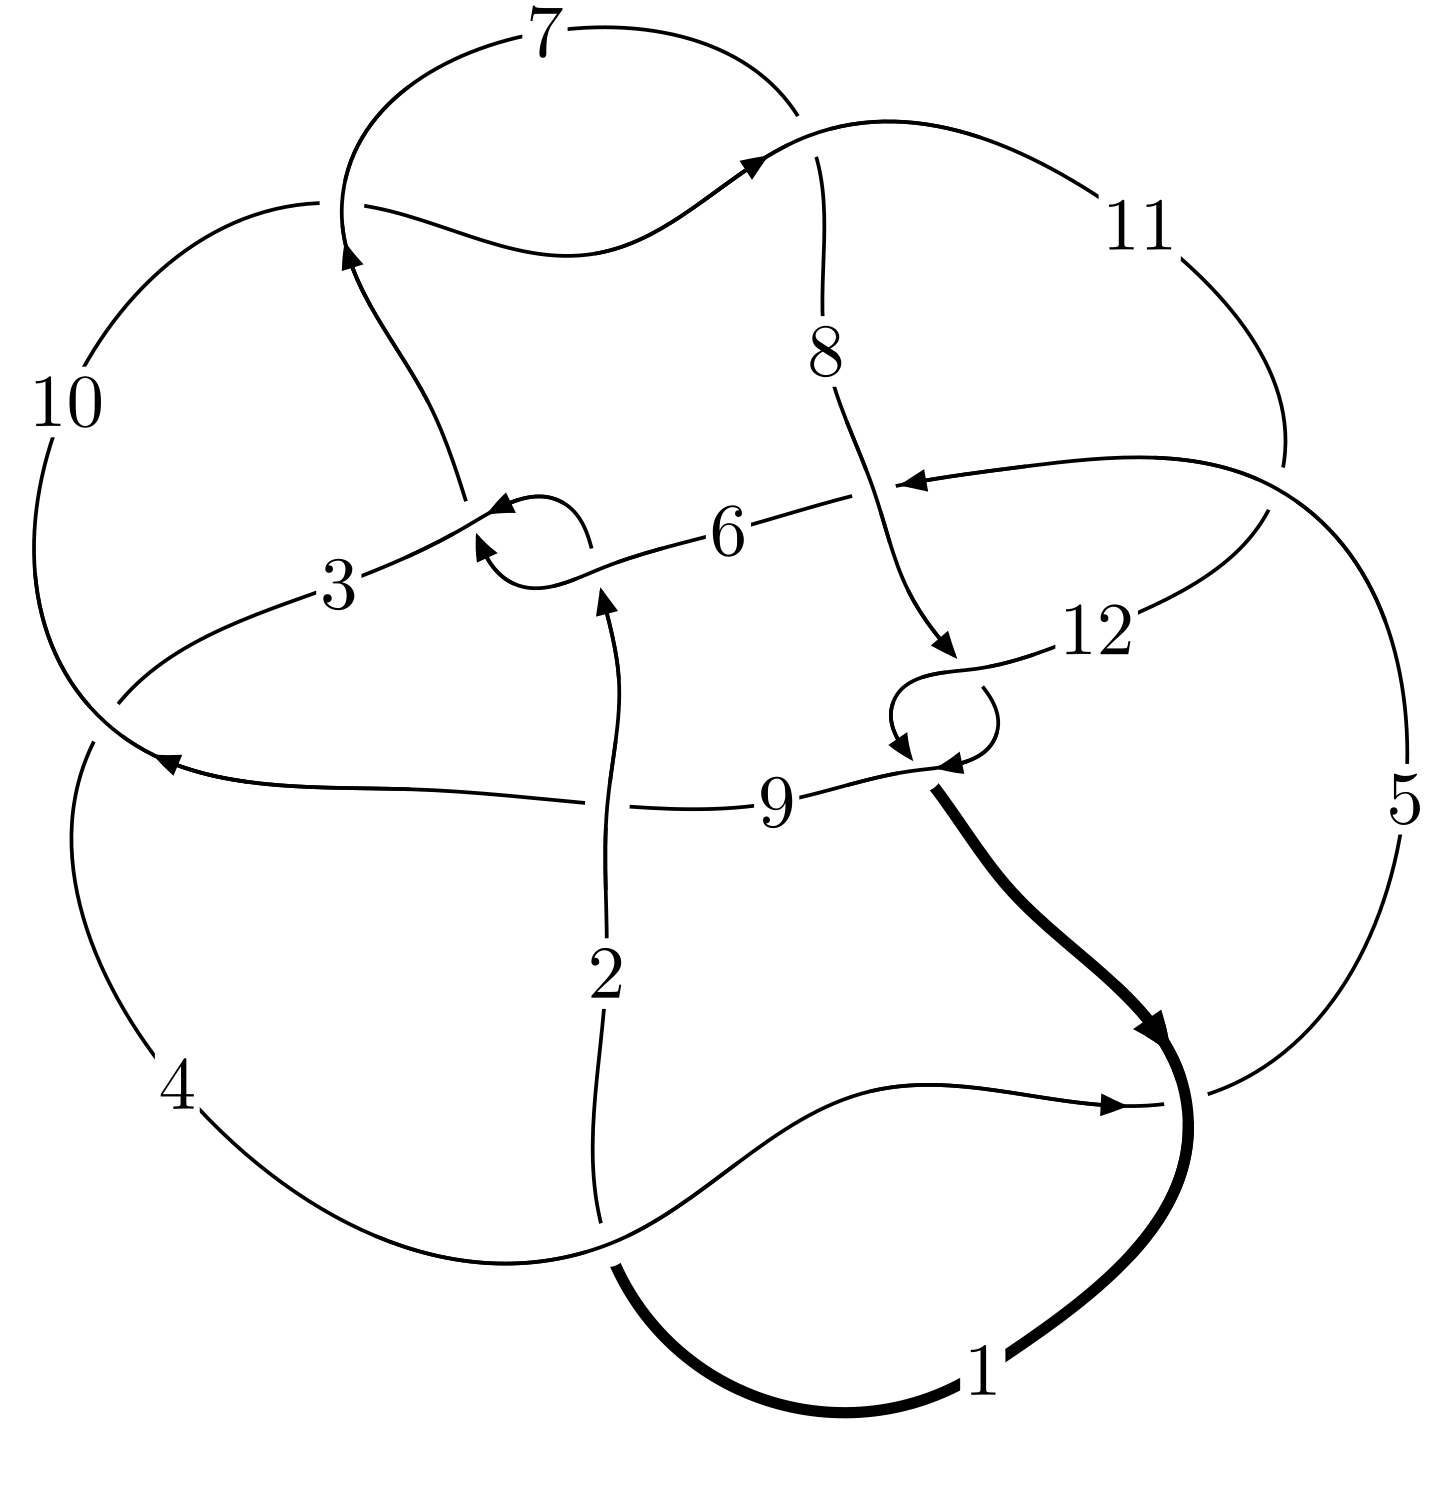
\includegraphics[width=112pt]{../../../GIT/diagram.site/Diagrams/png/1767_12a_0966.png}\\
\ \ \ A knot diagram\footnotemark}&
\allowdisplaybreaks
\textbf{Linearized knot diagam} \\
\cline{2-2}
 &
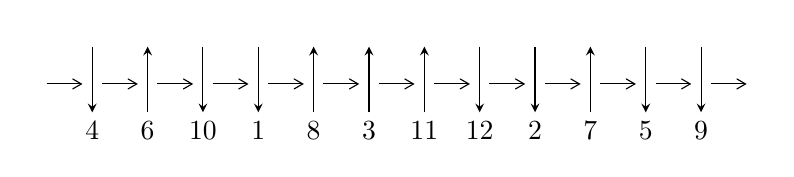
\begin{tikzpicture}[x=20pt, y=17pt]
	% nodes
	\node (C0) at (0, 0) {};
	\node (C1) at (1, 0) {};
	\node (C1U) at (1, +1) {};
	\node (C1D) at (1, -1) {4};

	\node (C2) at (2, 0) {};
	\node (C2U) at (2, +1) {};
	\node (C2D) at (2, -1) {6};

	\node (C3) at (3, 0) {};
	\node (C3U) at (3, +1) {};
	\node (C3D) at (3, -1) {10};

	\node (C4) at (4, 0) {};
	\node (C4U) at (4, +1) {};
	\node (C4D) at (4, -1) {1};

	\node (C5) at (5, 0) {};
	\node (C5U) at (5, +1) {};
	\node (C5D) at (5, -1) {8};

	\node (C6) at (6, 0) {};
	\node (C6U) at (6, +1) {};
	\node (C6D) at (6, -1) {3};

	\node (C7) at (7, 0) {};
	\node (C7U) at (7, +1) {};
	\node (C7D) at (7, -1) {11};

	\node (C8) at (8, 0) {};
	\node (C8U) at (8, +1) {};
	\node (C8D) at (8, -1) {12};

	\node (C9) at (9, 0) {};
	\node (C9U) at (9, +1) {};
	\node (C9D) at (9, -1) {2};

	\node (C10) at (10, 0) {};
	\node (C10U) at (10, +1) {};
	\node (C10D) at (10, -1) {7};

	\node (C11) at (11, 0) {};
	\node (C11U) at (11, +1) {};
	\node (C11D) at (11, -1) {5};

	\node (C12) at (12, 0) {};
	\node (C12U) at (12, +1) {};
	\node (C12D) at (12, -1) {9};
	\node (C13) at (13, 0) {};

	% arrows
	\draw[->,>={angle 60}]
	(C0) edge (C1) (C1) edge (C2) (C2) edge (C3) (C3) edge (C4) (C4) edge (C5) (C5) edge (C6) (C6) edge (C7) (C7) edge (C8) (C8) edge (C9) (C9) edge (C10) (C10) edge (C11) (C11) edge (C12) (C12) edge (C13) ;	\draw[->,>=stealth]
	(C1U) edge (C1D) (C2D) edge (C2U) (C3U) edge (C3D) (C4U) edge (C4D) (C5D) edge (C5U) (C6D) edge (C6U) (C7D) edge (C7U) (C8U) edge (C8D) (C9U) edge (C9D) (C10D) edge (C10U) (C11U) edge (C11D) (C12U) edge (C12D) ;
	\end{tikzpicture} \\
\hhline{~~} \\& 
\textbf{Solving Sequence} \\ \cline{2-2} 
 &
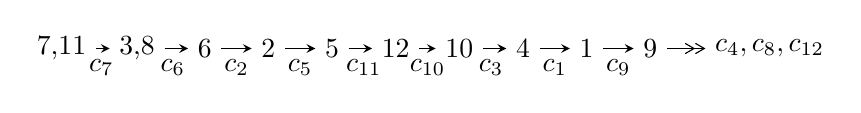
\begin{tikzpicture}[x=23pt, y=7pt]
	% node
	\node (A0) at (-1/8, 0) {7,11};
	\node (A1) at (17/16, 0) {3,8};
	\node (A2) at (17/8, 0) {6};
	\node (A3) at (25/8, 0) {2};
	\node (A4) at (33/8, 0) {5};
	\node (A5) at (41/8, 0) {12};
	\node (A6) at (49/8, 0) {10};
	\node (A7) at (57/8, 0) {4};
	\node (A8) at (65/8, 0) {1};
	\node (A9) at (73/8, 0) {9};
	\node (C1) at (1/2, -1) {$c_{7}$};
	\node (C2) at (13/8, -1) {$c_{6}$};
	\node (C3) at (21/8, -1) {$c_{2}$};
	\node (C4) at (29/8, -1) {$c_{5}$};
	\node (C5) at (37/8, -1) {$c_{11}$};
	\node (C6) at (45/8, -1) {$c_{10}$};
	\node (C7) at (53/8, -1) {$c_{3}$};
	\node (C8) at (61/8, -1) {$c_{1}$};
	\node (C9) at (69/8, -1) {$c_{9}$};
	\node (A10) at (11, 0) {$c_{4},c_{8},c_{12}$};

	% edge
	\draw[->,>=stealth]	
	(A0) edge (A1) (A1) edge (A2) (A2) edge (A3) (A3) edge (A4) (A4) edge (A5) (A5) edge (A6) (A6) edge (A7) (A7) edge (A8) (A8) edge (A9) ;
	\draw[->>,>={angle 60}]	
	(A9) edge (A10);
\end{tikzpicture} \\ 

\end{tabular} \\

\footnotetext{
The image of knot diagram is generated by the software ``\textbf{Draw programme}" developed by Andrew Bartholomew(\url{http://www.layer8.co.uk/maths/draw/index.htm\#Running-draw}), where we modified some parts for our purpose(\url{https://github.com/CATsTAILs/LinksPainter}).
}\phantom \\ \newline 
\centering \textbf{Ideals for irreducible components\footnotemark of $X_{\text{par}}$} 
 
\begin{align*}
I^u_{1}&=\langle 
-2.56009\times10^{774} u^{144}-4.93211\times10^{774} u^{143}+\cdots+1.27336\times10^{777} b-7.55766\times10^{778},\\
\phantom{I^u_{1}}&\phantom{= \langle  }7.70525\times10^{778} u^{144}+1.46879\times10^{779} u^{143}+\cdots+2.51680\times10^{781} a+2.16461\times10^{783},\\
\phantom{I^u_{1}}&\phantom{= \langle  }u^{145}+3 u^{144}+\cdots+45520 u+31624\rangle \\
I^u_{2}&=\langle 
2.15856\times10^{34} u^{36}-4.92672\times10^{34} u^{35}+\cdots+6.17494\times10^{32} b+7.43093\times10^{34},\\
\phantom{I^u_{2}}&\phantom{= \langle  }-1.17912\times10^{35} u^{36}+2.70674\times10^{35} u^{35}+\cdots+6.17494\times10^{32} a-3.94814\times10^{35},\\
\phantom{I^u_{2}}&\phantom{= \langle  }u^{37}-2 u^{36}+\cdots+10 u+1\rangle \\
\\
\end{align*}
\raggedright * 2 irreducible components of $\dim_{\mathbb{C}}=0$, with total 182 representations.\\
\footnotetext{All coefficients of polynomials are rational numbers. But the coefficients are sometimes approximated in decimal forms when there is not enough margin.}
\newpage
\renewcommand{\arraystretch}{1}
\centering \section*{I. $I^u_{1}= \langle -2.56\times10^{774} u^{144}-4.93\times10^{774} u^{143}+\cdots+1.27\times10^{777} b-7.56\times10^{778},\;7.71\times10^{778} u^{144}+1.47\times10^{779} u^{143}+\cdots+2.52\times10^{781} a+2.16\times10^{783},\;u^{145}+3 u^{144}+\cdots+45520 u+31624 \rangle$}
\flushleft \textbf{(i) Arc colorings}\\
\begin{tabular}{m{7pt} m{180pt} m{7pt} m{180pt} }
\flushright $a_{7}=$&$\begin{pmatrix}1\\0\end{pmatrix}$ \\
\flushright $a_{11}=$&$\begin{pmatrix}0\\u\end{pmatrix}$ \\
\flushright $a_{3}=$&$\begin{pmatrix}-0.00306152 u^{144}-0.00583593 u^{143}+\cdots-54.0993 u-86.0064\\0.00201049 u^{144}+0.00387329 u^{143}+\cdots+27.7562 u+59.3519\end{pmatrix}$ \\
\flushright $a_{8}=$&$\begin{pmatrix}1\\- u^2\end{pmatrix}$ \\
\flushright $a_{6}=$&$\begin{pmatrix}-0.00456419 u^{144}-0.00868214 u^{143}+\cdots-78.8377 u-129.918\\0.00349042 u^{144}+0.00666788 u^{143}+\cdots+48.4215 u+101.046\end{pmatrix}$ \\
\flushright $a_{2}=$&$\begin{pmatrix}-0.00105920 u^{144}-0.00215403 u^{143}+\cdots-11.3100 u-29.7437\\0.00177943 u^{144}+0.00349630 u^{143}+\cdots+30.1124 u+55.7141\end{pmatrix}$ \\
\flushright $a_{5}=$&$\begin{pmatrix}-0.00251406 u^{144}-0.00483637 u^{143}+\cdots-43.5228 u-72.5143\\0.000909316 u^{144}+0.00183026 u^{143}+\cdots+8.34863 u+28.1649\end{pmatrix}$ \\
\flushright $a_{12}=$&$\begin{pmatrix}-0.00500728 u^{144}-0.00958862 u^{143}+\cdots-81.4466 u-146.050\\0.00703064 u^{144}+0.0135010 u^{143}+\cdots+106.729 u+203.503\end{pmatrix}$ \\
\flushright $a_{10}=$&$\begin{pmatrix}- u\\u\end{pmatrix}$ \\
\flushright $a_{4}=$&$\begin{pmatrix}-0.00166098 u^{144}-0.00325291 u^{143}+\cdots-33.1480 u-48.3599\\0.000609948 u^{144}+0.00129027 u^{143}+\cdots+6.80493 u+21.7054\end{pmatrix}$ \\
\flushright $a_{1}=$&$\begin{pmatrix}-0.00143737 u^{144}-0.00285119 u^{143}+\cdots-12.1245 u-38.8485\\0.00199037 u^{144}+0.00385952 u^{143}+\cdots+30.0882 u+59.1760\end{pmatrix}$ \\
\flushright $a_{9}=$&$\begin{pmatrix}0.00649305 u^{144}+0.0125521 u^{143}+\cdots+83.6514 u+190.049\\-0.00867309 u^{144}-0.0167045 u^{143}+\cdots-122.458 u-250.360\end{pmatrix}$\\&\end{tabular}
\flushleft \textbf{(ii) Obstruction class $= -1$}\\~\\
\flushleft \textbf{(iii) Cusp Shapes $= 0.0461581 u^{144}+0.0859078 u^{143}+\cdots+728.816 u+1313.22$}\\~\\
\newpage\renewcommand{\arraystretch}{1}
\flushleft \textbf{(iv) u-Polynomials at the component}\newline \\
\begin{tabular}{m{50pt}|m{274pt}}
Crossings & \hspace{64pt}u-Polynomials at each crossing \\
\hline $$\begin{aligned}c_{1},c_{4}\end{aligned}$$&$\begin{aligned}
&u^{145}-10 u^{144}+\cdots-5940 u+449
\end{aligned}$\\
\hline $$\begin{aligned}c_{2},c_{6}\end{aligned}$$&$\begin{aligned}
&u^{145}-3 u^{144}+\cdots+467400 u-213397
\end{aligned}$\\
\hline $$\begin{aligned}c_{3}\end{aligned}$$&$\begin{aligned}
&u^{145}+u^{144}+\cdots-1175510402 u+376846879
\end{aligned}$\\
\hline $$\begin{aligned}c_{5}\end{aligned}$$&$\begin{aligned}
&u^{145}+13 u^{144}+\cdots+43 u+1
\end{aligned}$\\
\hline $$\begin{aligned}c_{7},c_{10}\end{aligned}$$&$\begin{aligned}
&u^{145}-3 u^{144}+\cdots+45520 u-31624
\end{aligned}$\\
\hline $$\begin{aligned}c_{8},c_{12}\end{aligned}$$&$\begin{aligned}
&u^{145}-47 u^{143}+\cdots-910 u+31
\end{aligned}$\\
\hline $$\begin{aligned}c_{9}\end{aligned}$$&$\begin{aligned}
&u^{145}-3 u^{144}+\cdots+64828 u+97949
\end{aligned}$\\
\hline $$\begin{aligned}c_{11}\end{aligned}$$&$\begin{aligned}
&u^{145}+2 u^{144}+\cdots-2298 u+229
\end{aligned}$\\
\hline
\end{tabular}\\~\\
\newpage\renewcommand{\arraystretch}{1}
\flushleft \textbf{(v) Riley Polynomials at the component}\newline \\
\begin{tabular}{m{50pt}|m{274pt}}
Crossings & \hspace{64pt}Riley Polynomials at each crossing \\
\hline $$\begin{aligned}c_{1},c_{4}\end{aligned}$$&$\begin{aligned}
&y^{145}+108 y^{144}+\cdots+3274390 y-201601
\end{aligned}$\\
\hline $$\begin{aligned}c_{2},c_{6}\end{aligned}$$&$\begin{aligned}
&y^{145}-95 y^{144}+\cdots+820020367120 y-45538279609
\end{aligned}$\\
\hline $$\begin{aligned}c_{3}\end{aligned}$$&$\begin{aligned}
&y^{145}+59 y^{144}+\cdots-6.17\times10^{18} y-1.42\times10^{17}
\end{aligned}$\\
\hline $$\begin{aligned}c_{5}\end{aligned}$$&$\begin{aligned}
&y^{145}+3 y^{144}+\cdots+517 y-1
\end{aligned}$\\
\hline $$\begin{aligned}c_{7},c_{10}\end{aligned}$$&$\begin{aligned}
&y^{145}-121 y^{144}+\cdots+10721993376 y-1000077376
\end{aligned}$\\
\hline $$\begin{aligned}c_{8},c_{12}\end{aligned}$$&$\begin{aligned}
&y^{145}-94 y^{144}+\cdots+537754 y-961
\end{aligned}$\\
\hline $$\begin{aligned}c_{9}\end{aligned}$$&$\begin{aligned}
&y^{145}+9 y^{144}+\cdots-357137656050 y-9594006601
\end{aligned}$\\
\hline $$\begin{aligned}c_{11}\end{aligned}$$&$\begin{aligned}
&y^{145}+28 y^{144}+\cdots-3337382 y-52441
\end{aligned}$\\
\hline
\end{tabular}\\~\\
\newpage\flushleft \textbf{(vi) Complex Volumes and Cusp Shapes}
$$\begin{array}{c|c|c}  
\text{Solutions to }I^u_{1}& \I (\text{vol} + \sqrt{-1}CS) & \text{Cusp shape}\\
 \hline 
\begin{aligned}
u &= \phantom{-}0.432137 + 0.929071 I \\
a &= \phantom{-}0.247856 - 0.672877 I \\
b &= -0.607437 - 0.431087 I\end{aligned}
 & -1.50937 - 2.56558 I & \phantom{-0.000000 } 0 \\ \hline\begin{aligned}
u &= \phantom{-}0.432137 - 0.929071 I \\
a &= \phantom{-}0.247856 + 0.672877 I \\
b &= -0.607437 + 0.431087 I\end{aligned}
 & -1.50937 + 2.56558 I & \phantom{-0.000000 } 0 \\ \hline\begin{aligned}
u &= \phantom{-}0.991744 + 0.289105 I \\
a &= -0.592041 - 0.027853 I \\
b &= \phantom{-}0.634555 + 0.969010 I\end{aligned}
 & \phantom{-}0.41359 + 3.40332 I & \phantom{-0.000000 } 0 \\ \hline\begin{aligned}
u &= \phantom{-}0.991744 - 0.289105 I \\
a &= -0.592041 + 0.027853 I \\
b &= \phantom{-}0.634555 - 0.969010 I\end{aligned}
 & \phantom{-}0.41359 - 3.40332 I & \phantom{-0.000000 } 0 \\ \hline\begin{aligned}
u &= \phantom{-}1.03384\phantom{ +0.000000I} \\
a &= \phantom{-}1.47451\phantom{ +0.000000I} \\
b &= -0.587025\phantom{ +0.000000I}\end{aligned}
 & -2.17833\phantom{ +0.000000I} & \phantom{-0.000000 } 0 \\ \hline\begin{aligned}
u &= \phantom{-}0.149129 + 1.045970 I \\
a &= \phantom{-}0.276971 - 0.214020 I \\
b &= -1.271740 + 0.272259 I\end{aligned}
 & \phantom{-}2.86533 - 2.84293 I & \phantom{-0.000000 } 0 \\ \hline\begin{aligned}
u &= \phantom{-}0.149129 - 1.045970 I \\
a &= \phantom{-}0.276971 + 0.214020 I \\
b &= -1.271740 - 0.272259 I\end{aligned}
 & \phantom{-}2.86533 + 2.84293 I & \phantom{-0.000000 } 0 \\ \hline\begin{aligned}
u &= \phantom{-}0.402800 + 0.979557 I \\
a &= \phantom{-}0.537460 - 0.320233 I \\
b &= -1.087970 - 0.500347 I\end{aligned}
 & -3.43730 + 7.78539 I & \phantom{-0.000000 } 0 \\ \hline\begin{aligned}
u &= \phantom{-}0.402800 - 0.979557 I \\
a &= \phantom{-}0.537460 + 0.320233 I \\
b &= -1.087970 + 0.500347 I\end{aligned}
 & -3.43730 - 7.78539 I & \phantom{-0.000000 } 0 \\ \hline\begin{aligned}
u &= -1.039170 + 0.257462 I \\
a &= \phantom{-}0.187116 - 0.253724 I \\
b &= \phantom{-}0.138445 - 0.388984 I\end{aligned}
 & \phantom{-}1.80222 - 1.09093 I & \phantom{-0.000000 } 0\\
 \hline 
 \end{array}$$\newpage$$\begin{array}{c|c|c}  
\text{Solutions to }I^u_{1}& \I (\text{vol} + \sqrt{-1}CS) & \text{Cusp shape}\\
 \hline 
\begin{aligned}
u &= -1.039170 - 0.257462 I \\
a &= \phantom{-}0.187116 + 0.253724 I \\
b &= \phantom{-}0.138445 + 0.388984 I\end{aligned}
 & \phantom{-}1.80222 + 1.09093 I & \phantom{-0.000000 } 0 \\ \hline\begin{aligned}
u &= -0.381911 + 1.002350 I \\
a &= \phantom{-}0.238783 + 0.567284 I \\
b &= -1.232410 - 0.366256 I\end{aligned}
 & \phantom{-}2.32411 + 4.31465 I & \phantom{-0.000000 } 0 \\ \hline\begin{aligned}
u &= -0.381911 - 1.002350 I \\
a &= \phantom{-}0.238783 - 0.567284 I \\
b &= -1.232410 + 0.366256 I\end{aligned}
 & \phantom{-}2.32411 - 4.31465 I & \phantom{-0.000000 } 0 \\ \hline\begin{aligned}
u &= -1.080430 + 0.017548 I \\
a &= -0.456845 - 0.597509 I \\
b &= \phantom{-}0.37817 + 1.47138 I\end{aligned}
 & -1.37218 + 2.69986 I & \phantom{-0.000000 } 0 \\ \hline\begin{aligned}
u &= -1.080430 - 0.017548 I \\
a &= -0.456845 + 0.597509 I \\
b &= \phantom{-}0.37817 - 1.47138 I\end{aligned}
 & -1.37218 - 2.69986 I & \phantom{-0.000000 } 0 \\ \hline\begin{aligned}
u &= -0.732863 + 0.518690 I \\
a &= \phantom{-}1.199190 - 0.622697 I \\
b &= -0.177234 + 0.625707 I\end{aligned}
 & -1.034490 + 0.537752 I & \phantom{-0.000000 } 0 \\ \hline\begin{aligned}
u &= -0.732863 - 0.518690 I \\
a &= \phantom{-}1.199190 + 0.622697 I \\
b &= -0.177234 - 0.625707 I\end{aligned}
 & -1.034490 - 0.537752 I & \phantom{-0.000000 } 0 \\ \hline\begin{aligned}
u &= \phantom{-}0.886943 + 0.068598 I \\
a &= -2.26071 + 0.57400 I \\
b &= \phantom{-}1.021750 - 0.324888 I\end{aligned}
 & \phantom{-}1.22023 - 3.51637 I & \phantom{-0.000000 } 0 \\ \hline\begin{aligned}
u &= \phantom{-}0.886943 - 0.068598 I \\
a &= -2.26071 - 0.57400 I \\
b &= \phantom{-}1.021750 + 0.324888 I\end{aligned}
 & \phantom{-}1.22023 + 3.51637 I & \phantom{-0.000000 } 0 \\ \hline\begin{aligned}
u &= -1.13193\phantom{ +0.000000I} \\
a &= -3.43344\phantom{ +0.000000I} \\
b &= \phantom{-}1.13104\phantom{ +0.000000I}\end{aligned}
 & \phantom{-}3.81621\phantom{ +0.000000I} & \phantom{-0.000000 } 0\\
 \hline 
 \end{array}$$\newpage$$\begin{array}{c|c|c}  
\text{Solutions to }I^u_{1}& \I (\text{vol} + \sqrt{-1}CS) & \text{Cusp shape}\\
 \hline 
\begin{aligned}
u &= \phantom{-}0.273319 + 0.811271 I \\
a &= \phantom{-}0.896255 + 1.017420 I \\
b &= -0.839346 + 0.550520 I\end{aligned}
 & -1.00479 - 6.66392 I & \phantom{-0.000000 } 0 \\ \hline\begin{aligned}
u &= \phantom{-}0.273319 - 0.811271 I \\
a &= \phantom{-}0.896255 - 1.017420 I \\
b &= -0.839346 - 0.550520 I\end{aligned}
 & -1.00479 + 6.66392 I & \phantom{-0.000000 } 0 \\ \hline\begin{aligned}
u &= -0.347323 + 1.094070 I \\
a &= \phantom{-}0.538236 + 0.260578 I \\
b &= -1.041790 + 0.280004 I\end{aligned}
 & \phantom{-}1.20505 - 3.57769 I & \phantom{-0.000000 } 0 \\ \hline\begin{aligned}
u &= -0.347323 - 1.094070 I \\
a &= \phantom{-}0.538236 - 0.260578 I \\
b &= -1.041790 - 0.280004 I\end{aligned}
 & \phantom{-}1.20505 + 3.57769 I & \phantom{-0.000000 } 0 \\ \hline\begin{aligned}
u &= \phantom{-}0.292275 + 0.792638 I \\
a &= \phantom{-}0.320226 + 0.396084 I \\
b &= \phantom{-}0.920455 + 0.417485 I\end{aligned}
 & -2.99660 + 1.39102 I & \phantom{-0.000000 } 0 \\ \hline\begin{aligned}
u &= \phantom{-}0.292275 - 0.792638 I \\
a &= \phantom{-}0.320226 - 0.396084 I \\
b &= \phantom{-}0.920455 - 0.417485 I\end{aligned}
 & -2.99660 - 1.39102 I & \phantom{-0.000000 } 0 \\ \hline\begin{aligned}
u &= -1.168920 + 0.064116 I \\
a &= -2.87834 + 0.11170 I \\
b &= \phantom{-}1.102830 + 0.016813 I\end{aligned}
 & \phantom{-}3.71741 - 0.14086 I & \phantom{-0.000000 } 0 \\ \hline\begin{aligned}
u &= -1.168920 - 0.064116 I \\
a &= -2.87834 - 0.11170 I \\
b &= \phantom{-}1.102830 - 0.016813 I\end{aligned}
 & \phantom{-}3.71741 + 0.14086 I & \phantom{-0.000000 } 0 \\ \hline\begin{aligned}
u &= -0.149563 + 0.802553 I \\
a &= -0.933196 + 0.879312 I \\
b &= \phantom{-}0.217325 + 0.403873 I\end{aligned}
 & \phantom{-}2.66849 - 2.92410 I & \phantom{-0.000000 } 0 \\ \hline\begin{aligned}
u &= -0.149563 - 0.802553 I \\
a &= -0.933196 - 0.879312 I \\
b &= \phantom{-}0.217325 - 0.403873 I\end{aligned}
 & \phantom{-}2.66849 + 2.92410 I & \phantom{-0.000000 } 0\\
 \hline 
 \end{array}$$\newpage$$\begin{array}{c|c|c}  
\text{Solutions to }I^u_{1}& \I (\text{vol} + \sqrt{-1}CS) & \text{Cusp shape}\\
 \hline 
\begin{aligned}
u &= -0.194598 + 1.169750 I \\
a &= -0.373847 + 0.251540 I \\
b &= \phantom{-}1.169130 - 0.018165 I\end{aligned}
 & \phantom{-}3.29951 - 2.40492 I & \phantom{-0.000000 } 0 \\ \hline\begin{aligned}
u &= -0.194598 - 1.169750 I \\
a &= -0.373847 - 0.251540 I \\
b &= \phantom{-}1.169130 + 0.018165 I\end{aligned}
 & \phantom{-}3.29951 + 2.40492 I & \phantom{-0.000000 } 0 \\ \hline\begin{aligned}
u &= -0.799508 + 0.132155 I \\
a &= \phantom{-}1.037660 + 0.001514 I \\
b &= \phantom{-}0.723394 - 0.126628 I\end{aligned}
 & \phantom{-}2.31491 - 0.53337 I & \phantom{-0.000000 } 0 \\ \hline\begin{aligned}
u &= -0.799508 - 0.132155 I \\
a &= \phantom{-}1.037660 - 0.001514 I \\
b &= \phantom{-}0.723394 + 0.126628 I\end{aligned}
 & \phantom{-}2.31491 + 0.53337 I & \phantom{-0.000000 } 0 \\ \hline\begin{aligned}
u &= \phantom{-}1.181860 + 0.154851 I \\
a &= \phantom{-}0.596951 + 0.002605 I \\
b &= -0.82914 - 1.15633 I\end{aligned}
 & \phantom{-}0.46658 + 3.93656 I & \phantom{-0.000000 } 0 \\ \hline\begin{aligned}
u &= \phantom{-}1.181860 - 0.154851 I \\
a &= \phantom{-}0.596951 - 0.002605 I \\
b &= -0.82914 + 1.15633 I\end{aligned}
 & \phantom{-}0.46658 - 3.93656 I & \phantom{-0.000000 } 0 \\ \hline\begin{aligned}
u &= -0.951518 + 0.725435 I \\
a &= \phantom{-}0.020359 - 0.422169 I \\
b &= -0.688451 - 0.422754 I\end{aligned}
 & \phantom{-}3.88447 - 1.34262 I & \phantom{-0.000000 } 0 \\ \hline\begin{aligned}
u &= -0.951518 - 0.725435 I \\
a &= \phantom{-}0.020359 + 0.422169 I \\
b &= -0.688451 + 0.422754 I\end{aligned}
 & \phantom{-}3.88447 + 1.34262 I & \phantom{-0.000000 } 0 \\ \hline\begin{aligned}
u &= \phantom{-}0.111251 + 0.784602 I \\
a &= -1.191210 - 0.562088 I \\
b &= \phantom{-}0.298123 - 0.717683 I\end{aligned}
 & -1.57095 + 8.78124 I & \phantom{-0.000000 } 0 \\ \hline\begin{aligned}
u &= \phantom{-}0.111251 - 0.784602 I \\
a &= -1.191210 + 0.562088 I \\
b &= \phantom{-}0.298123 + 0.717683 I\end{aligned}
 & -1.57095 - 8.78124 I & \phantom{-0.000000 } 0\\
 \hline 
 \end{array}$$\newpage$$\begin{array}{c|c|c}  
\text{Solutions to }I^u_{1}& \I (\text{vol} + \sqrt{-1}CS) & \text{Cusp shape}\\
 \hline 
\begin{aligned}
u &= \phantom{-}1.088150 + 0.566831 I \\
a &= -0.120615 + 0.608113 I \\
b &= \phantom{-}0.761839 + 0.016293 I\end{aligned}
 & -0.69185 + 3.63054 I & \phantom{-0.000000 } 0 \\ \hline\begin{aligned}
u &= \phantom{-}1.088150 - 0.566831 I \\
a &= -0.120615 - 0.608113 I \\
b &= \phantom{-}0.761839 - 0.016293 I\end{aligned}
 & -0.69185 - 3.63054 I & \phantom{-0.000000 } 0 \\ \hline\begin{aligned}
u &= \phantom{-}1.219060 + 0.162674 I \\
a &= -0.138189 - 0.470608 I \\
b &= \phantom{-}0.073557 + 1.204540 I\end{aligned}
 & \phantom{-}2.00915 + 3.11835 I & \phantom{-0.000000 } 0 \\ \hline\begin{aligned}
u &= \phantom{-}1.219060 - 0.162674 I \\
a &= -0.138189 + 0.470608 I \\
b &= \phantom{-}0.073557 - 1.204540 I\end{aligned}
 & \phantom{-}2.00915 - 3.11835 I & \phantom{-0.000000 } 0 \\ \hline\begin{aligned}
u &= \phantom{-}0.611605 + 0.457951 I \\
a &= \phantom{-}0.30112 - 1.62200 I \\
b &= -0.597573 + 0.431575 I\end{aligned}
 & -1.45105 - 1.92208 I & \phantom{-0.000000 } 0 \\ \hline\begin{aligned}
u &= \phantom{-}0.611605 - 0.457951 I \\
a &= \phantom{-}0.30112 + 1.62200 I \\
b &= -0.597573 - 0.431575 I\end{aligned}
 & -1.45105 + 1.92208 I & \phantom{-0.000000 } 0 \\ \hline\begin{aligned}
u &= -1.240890 + 0.066673 I \\
a &= -2.14499 - 0.72682 I \\
b &= \phantom{-}1.42229 - 0.26765 I\end{aligned}
 & \phantom{-}5.11259 + 0.43687 I & \phantom{-0.000000 } 0 \\ \hline\begin{aligned}
u &= -1.240890 - 0.066673 I \\
a &= -2.14499 + 0.72682 I \\
b &= \phantom{-}1.42229 + 0.26765 I\end{aligned}
 & \phantom{-}5.11259 - 0.43687 I & \phantom{-0.000000 } 0 \\ \hline\begin{aligned}
u &= \phantom{-}1.074680 + 0.629418 I \\
a &= -0.220650 - 0.203125 I \\
b &= -0.532007 + 0.390425 I\end{aligned}
 & \phantom{-}0.48860 + 8.13399 I & \phantom{-0.000000 } 0 \\ \hline\begin{aligned}
u &= \phantom{-}1.074680 - 0.629418 I \\
a &= -0.220650 + 0.203125 I \\
b &= -0.532007 - 0.390425 I\end{aligned}
 & \phantom{-}0.48860 - 8.13399 I & \phantom{-0.000000 } 0\\
 \hline 
 \end{array}$$\newpage$$\begin{array}{c|c|c}  
\text{Solutions to }I^u_{1}& \I (\text{vol} + \sqrt{-1}CS) & \text{Cusp shape}\\
 \hline 
\begin{aligned}
u &= \phantom{-}1.25636\phantom{ +0.000000I} \\
a &= \phantom{-}1.61669\phantom{ +0.000000I} \\
b &= -0.809048\phantom{ +0.000000I}\end{aligned}
 & -2.14218\phantom{ +0.000000I} & \phantom{-0.000000 } 0 \\ \hline\begin{aligned}
u &= \phantom{-}0.972639 + 0.809961 I \\
a &= \phantom{-}0.706308 - 0.545033 I \\
b &= -0.842407 + 0.184630 I\end{aligned}
 & -1.89215 - 1.74159 I & \phantom{-0.000000 } 0 \\ \hline\begin{aligned}
u &= \phantom{-}0.972639 - 0.809961 I \\
a &= \phantom{-}0.706308 + 0.545033 I \\
b &= -0.842407 - 0.184630 I\end{aligned}
 & -1.89215 + 1.74159 I & \phantom{-0.000000 } 0 \\ \hline\begin{aligned}
u &= -1.253380 + 0.201642 I \\
a &= \phantom{-}1.45086 + 1.08106 I \\
b &= -1.249390 + 0.495735 I\end{aligned}
 & \phantom{-}9.78521 - 4.73385 I & \phantom{-0.000000 } 0 \\ \hline\begin{aligned}
u &= -1.253380 - 0.201642 I \\
a &= \phantom{-}1.45086 - 1.08106 I \\
b &= -1.249390 - 0.495735 I\end{aligned}
 & \phantom{-}9.78521 + 4.73385 I & \phantom{-0.000000 } 0 \\ \hline\begin{aligned}
u &= -1.186680 + 0.465651 I \\
a &= \phantom{-}1.61366 + 0.58709 I \\
b &= -1.56132 + 0.55391 I\end{aligned}
 & \phantom{-}4.94868 - 9.60654 I & \phantom{-0.000000 } 0 \\ \hline\begin{aligned}
u &= -1.186680 - 0.465651 I \\
a &= \phantom{-}1.61366 - 0.58709 I \\
b &= -1.56132 - 0.55391 I\end{aligned}
 & \phantom{-}4.94868 + 9.60654 I & \phantom{-0.000000 } 0 \\ \hline\begin{aligned}
u &= \phantom{-}1.245260 + 0.300384 I \\
a &= \phantom{-}2.52820 - 0.27465 I \\
b &= -1.083010 - 0.202793 I\end{aligned}
 & \phantom{-}2.14223 + 10.50550 I & \phantom{-0.000000 } 0 \\ \hline\begin{aligned}
u &= \phantom{-}1.245260 - 0.300384 I \\
a &= \phantom{-}2.52820 + 0.27465 I \\
b &= -1.083010 + 0.202793 I\end{aligned}
 & \phantom{-}2.14223 - 10.50550 I & \phantom{-0.000000 } 0 \\ \hline\begin{aligned}
u &= -1.288440 + 0.164268 I \\
a &= -0.290308 + 0.074632 I \\
b &= -0.199417 + 0.815441 I\end{aligned}
 & \phantom{-}6.54945 - 0.16529 I & \phantom{-0.000000 } 0\\
 \hline 
 \end{array}$$\newpage$$\begin{array}{c|c|c}  
\text{Solutions to }I^u_{1}& \I (\text{vol} + \sqrt{-1}CS) & \text{Cusp shape}\\
 \hline 
\begin{aligned}
u &= -1.288440 - 0.164268 I \\
a &= -0.290308 - 0.074632 I \\
b &= -0.199417 - 0.815441 I\end{aligned}
 & \phantom{-}6.54945 + 0.16529 I & \phantom{-0.000000 } 0 \\ \hline\begin{aligned}
u &= \phantom{-}0.423131 + 0.558136 I \\
a &= \phantom{-}1.023360 + 0.451687 I \\
b &= \phantom{-}0.123736 - 0.552332 I\end{aligned}
 & -1.282110 + 0.180959 I & \phantom{-0.000000 } 0 \\ \hline\begin{aligned}
u &= \phantom{-}0.423131 - 0.558136 I \\
a &= \phantom{-}1.023360 - 0.451687 I \\
b &= \phantom{-}0.123736 + 0.552332 I\end{aligned}
 & -1.282110 - 0.180959 I & \phantom{-0.000000 } 0 \\ \hline\begin{aligned}
u &= -1.238570 + 0.396683 I \\
a &= \phantom{-}2.04521 + 0.74013 I \\
b &= -1.044750 + 0.176164 I\end{aligned}
 & \phantom{-}4.89618 - 3.90342 I & \phantom{-0.000000 } 0 \\ \hline\begin{aligned}
u &= -1.238570 - 0.396683 I \\
a &= \phantom{-}2.04521 - 0.74013 I \\
b &= -1.044750 - 0.176164 I\end{aligned}
 & \phantom{-}4.89618 + 3.90342 I & \phantom{-0.000000 } 0 \\ \hline\begin{aligned}
u &= \phantom{-}1.309130 + 0.130866 I \\
a &= -2.37394 - 0.54205 I \\
b &= \phantom{-}1.073950 + 0.077491 I\end{aligned}
 & \phantom{-}0.47115 + 4.19298 I & \phantom{-0.000000 } 0 \\ \hline\begin{aligned}
u &= \phantom{-}1.309130 - 0.130866 I \\
a &= -2.37394 + 0.54205 I \\
b &= \phantom{-}1.073950 - 0.077491 I\end{aligned}
 & \phantom{-}0.47115 - 4.19298 I & \phantom{-0.000000 } 0 \\ \hline\begin{aligned}
u &= -1.322570 + 0.032054 I \\
a &= \phantom{-}1.78071 + 0.35786 I \\
b &= -1.61570 + 0.41951 I\end{aligned}
 & \phantom{-}8.93479 + 6.21741 I & \phantom{-0.000000 } 0 \\ \hline\begin{aligned}
u &= -1.322570 - 0.032054 I \\
a &= \phantom{-}1.78071 - 0.35786 I \\
b &= -1.61570 - 0.41951 I\end{aligned}
 & \phantom{-}8.93479 - 6.21741 I & \phantom{-0.000000 } 0 \\ \hline\begin{aligned}
u &= \phantom{-}1.320640 + 0.166718 I \\
a &= -1.80669 + 0.43155 I \\
b &= \phantom{-}1.43776 + 0.49720 I\end{aligned}
 & \phantom{-}6.68031 + 3.11471 I & \phantom{-0.000000 } 0\\
 \hline 
 \end{array}$$\newpage$$\begin{array}{c|c|c}  
\text{Solutions to }I^u_{1}& \I (\text{vol} + \sqrt{-1}CS) & \text{Cusp shape}\\
 \hline 
\begin{aligned}
u &= \phantom{-}1.320640 - 0.166718 I \\
a &= -1.80669 - 0.43155 I \\
b &= \phantom{-}1.43776 - 0.49720 I\end{aligned}
 & \phantom{-}6.68031 - 3.11471 I & \phantom{-0.000000 } 0 \\ \hline\begin{aligned}
u &= -1.322050 + 0.234961 I \\
a &= \phantom{-}0.130530 + 0.684390 I \\
b &= -0.189014 - 1.333740 I\end{aligned}
 & -1.34551 - 5.96775 I & \phantom{-0.000000 } 0 \\ \hline\begin{aligned}
u &= -1.322050 - 0.234961 I \\
a &= \phantom{-}0.130530 - 0.684390 I \\
b &= -0.189014 + 1.333740 I\end{aligned}
 & -1.34551 + 5.96775 I & \phantom{-0.000000 } 0 \\ \hline\begin{aligned}
u &= -1.317320 + 0.291863 I \\
a &= -1.49882 - 0.27319 I \\
b &= \phantom{-}1.36059 - 0.72046 I\end{aligned}
 & \phantom{-}1.93253 - 4.97336 I & \phantom{-0.000000 } 0 \\ \hline\begin{aligned}
u &= -1.317320 - 0.291863 I \\
a &= -1.49882 + 0.27319 I \\
b &= \phantom{-}1.36059 + 0.72046 I\end{aligned}
 & \phantom{-}1.93253 + 4.97336 I & \phantom{-0.000000 } 0 \\ \hline\begin{aligned}
u &= -1.315820 + 0.333200 I \\
a &= -0.009504 + 0.303187 I \\
b &= \phantom{-}0.231689 + 0.693846 I\end{aligned}
 & \phantom{-}4.07611 - 0.56137 I & \phantom{-0.000000 } 0 \\ \hline\begin{aligned}
u &= -1.315820 - 0.333200 I \\
a &= -0.009504 - 0.303187 I \\
b &= \phantom{-}0.231689 - 0.693846 I\end{aligned}
 & \phantom{-}4.07611 + 0.56137 I & \phantom{-0.000000 } 0 \\ \hline\begin{aligned}
u &= \phantom{-}1.340660 + 0.239843 I \\
a &= \phantom{-}1.79440 - 0.84942 I \\
b &= -1.40158 - 0.46257 I\end{aligned}
 & \phantom{-}9.16611 + 9.90378 I & \phantom{-0.000000 } 0 \\ \hline\begin{aligned}
u &= \phantom{-}1.340660 - 0.239843 I \\
a &= \phantom{-}1.79440 + 0.84942 I \\
b &= -1.40158 + 0.46257 I\end{aligned}
 & \phantom{-}9.16611 - 9.90378 I & \phantom{-0.000000 } 0 \\ \hline\begin{aligned}
u &= \phantom{-}0.044295 + 0.633256 I \\
a &= \phantom{-}0.956492 + 0.411775 I \\
b &= -0.397134 + 0.845440 I\end{aligned}
 & -5.62423 + 2.85523 I & \phantom{-0.000000 } 0\\
 \hline 
 \end{array}$$\newpage$$\begin{array}{c|c|c}  
\text{Solutions to }I^u_{1}& \I (\text{vol} + \sqrt{-1}CS) & \text{Cusp shape}\\
 \hline 
\begin{aligned}
u &= \phantom{-}0.044295 - 0.633256 I \\
a &= \phantom{-}0.956492 - 0.411775 I \\
b &= -0.397134 - 0.845440 I\end{aligned}
 & -5.62423 - 2.85523 I & \phantom{-0.000000 } 0 \\ \hline\begin{aligned}
u &= \phantom{-}1.384370 + 0.034051 I \\
a &= -0.556285 + 0.408484 I \\
b &= \phantom{-}0.248856 - 1.094270 I\end{aligned}
 & \phantom{-}4.07202 - 4.55213 I & \phantom{-0.000000 } 0 \\ \hline\begin{aligned}
u &= \phantom{-}1.384370 - 0.034051 I \\
a &= -0.556285 - 0.408484 I \\
b &= \phantom{-}0.248856 + 1.094270 I\end{aligned}
 & \phantom{-}4.07202 + 4.55213 I & \phantom{-0.000000 } 0 \\ \hline\begin{aligned}
u &= \phantom{-}0.430440 + 1.324000 I \\
a &= -0.523914 + 0.278125 I \\
b &= \phantom{-}1.171860 + 0.414606 I\end{aligned}
 & \phantom{-}1.17364 + 13.05360 I & \phantom{-0.000000 } 0 \\ \hline\begin{aligned}
u &= \phantom{-}0.430440 - 1.324000 I \\
a &= -0.523914 - 0.278125 I \\
b &= \phantom{-}1.171860 - 0.414606 I\end{aligned}
 & \phantom{-}1.17364 - 13.05360 I & \phantom{-0.000000 } 0 \\ \hline\begin{aligned}
u &= -0.600855 + 0.038418 I \\
a &= -1.31020 + 1.79200 I \\
b &= \phantom{-}0.809579 - 1.013760 I\end{aligned}
 & -2.91292 - 3.38530 I & -9.26974 + 8.26425 I \\ \hline\begin{aligned}
u &= -0.600855 - 0.038418 I \\
a &= -1.31020 - 1.79200 I \\
b &= \phantom{-}0.809579 + 1.013760 I\end{aligned}
 & -2.91292 + 3.38530 I & -9.26974 - 8.26425 I \\ \hline\begin{aligned}
u &= -1.369100 + 0.329860 I \\
a &= \phantom{-}0.020293 - 0.413861 I \\
b &= \phantom{-}0.095722 + 1.295860 I\end{aligned}
 & \phantom{-}3.16925 - 12.78880 I & \phantom{-0.000000 } 0 \\ \hline\begin{aligned}
u &= -1.369100 - 0.329860 I \\
a &= \phantom{-}0.020293 + 0.413861 I \\
b &= \phantom{-}0.095722 - 1.295860 I\end{aligned}
 & \phantom{-}3.16925 + 12.78880 I & \phantom{-0.000000 } 0 \\ \hline\begin{aligned}
u &= \phantom{-}0.579973 + 0.070200 I \\
a &= -0.781754 + 0.060310 I \\
b &= \phantom{-}0.905376 + 0.829679 I\end{aligned}
 & \phantom{-}0.55942 + 3.12092 I & \phantom{-}6.15818 - 7.11948 I\\
 \hline 
 \end{array}$$\newpage$$\begin{array}{c|c|c}  
\text{Solutions to }I^u_{1}& \I (\text{vol} + \sqrt{-1}CS) & \text{Cusp shape}\\
 \hline 
\begin{aligned}
u &= \phantom{-}0.579973 - 0.070200 I \\
a &= -0.781754 - 0.060310 I \\
b &= \phantom{-}0.905376 - 0.829679 I\end{aligned}
 & \phantom{-}0.55942 - 3.12092 I & \phantom{-}6.15818 + 7.11948 I \\ \hline\begin{aligned}
u &= \phantom{-}1.38642 + 0.32349 I \\
a &= \phantom{-}0.058091 + 0.191128 I \\
b &= \phantom{-}0.087256 - 1.097540 I\end{aligned}
 & \phantom{-}7.65844 + 6.95339 I & \phantom{-0.000000 } 0 \\ \hline\begin{aligned}
u &= \phantom{-}1.38642 - 0.32349 I \\
a &= \phantom{-}0.058091 - 0.191128 I \\
b &= \phantom{-}0.087256 + 1.097540 I\end{aligned}
 & \phantom{-}7.65844 - 6.95339 I & \phantom{-0.000000 } 0 \\ \hline\begin{aligned}
u &= \phantom{-}1.42622 + 0.03310 I \\
a &= \phantom{-}1.57260 - 0.30998 I \\
b &= -1.42383 - 0.46057 I\end{aligned}
 & \phantom{-}12.51670 - 1.37041 I & \phantom{-0.000000 } 0 \\ \hline\begin{aligned}
u &= \phantom{-}1.42622 - 0.03310 I \\
a &= \phantom{-}1.57260 + 0.30998 I \\
b &= -1.42383 + 0.46057 I\end{aligned}
 & \phantom{-}12.51670 + 1.37041 I & \phantom{-0.000000 } 0 \\ \hline\begin{aligned}
u &= \phantom{-}1.35792 + 0.49954 I \\
a &= \phantom{-}1.64429 - 0.58403 I \\
b &= -1.49592 - 0.43611 I\end{aligned}
 & \phantom{-}6.81907 + 8.41116 I & \phantom{-0.000000 } 0 \\ \hline\begin{aligned}
u &= \phantom{-}1.35792 - 0.49954 I \\
a &= \phantom{-}1.64429 + 0.58403 I \\
b &= -1.49592 + 0.43611 I\end{aligned}
 & \phantom{-}6.81907 - 8.41116 I & \phantom{-0.000000 } 0 \\ \hline\begin{aligned}
u &= \phantom{-}0.546114 + 0.061781 I \\
a &= -1.262060 - 0.442290 I \\
b &= \phantom{-}0.637608 + 0.715268 I\end{aligned}
 & \phantom{-}0.85329 + 2.27952 I & -4.05928 - 1.94360 I \\ \hline\begin{aligned}
u &= \phantom{-}0.546114 - 0.061781 I \\
a &= -1.262060 + 0.442290 I \\
b &= \phantom{-}0.637608 - 0.715268 I\end{aligned}
 & \phantom{-}0.85329 - 2.27952 I & -4.05928 + 1.94360 I \\ \hline\begin{aligned}
u &= \phantom{-}0.203415 + 0.494746 I \\
a &= \phantom{-}1.104620 - 0.378266 I \\
b &= -0.230332 - 0.453612 I\end{aligned}
 & -1.026120 - 0.579671 I & -8.11952 + 2.62937 I\\
 \hline 
 \end{array}$$\newpage$$\begin{array}{c|c|c}  
\text{Solutions to }I^u_{1}& \I (\text{vol} + \sqrt{-1}CS) & \text{Cusp shape}\\
 \hline 
\begin{aligned}
u &= \phantom{-}0.203415 - 0.494746 I \\
a &= \phantom{-}1.104620 + 0.378266 I \\
b &= -0.230332 + 0.453612 I\end{aligned}
 & -1.026120 + 0.579671 I & -8.11952 - 2.62937 I \\ \hline\begin{aligned}
u &= -0.394101 + 0.352701 I \\
a &= -0.414129 - 0.418438 I \\
b &= \phantom{-}0.301682 - 0.964513 I\end{aligned}
 & -1.55548 - 3.86108 I & -5.10180 + 9.95738 I \\ \hline\begin{aligned}
u &= -0.394101 - 0.352701 I \\
a &= -0.414129 + 0.418438 I \\
b &= \phantom{-}0.301682 + 0.964513 I\end{aligned}
 & -1.55548 + 3.86108 I & -5.10180 - 9.95738 I \\ \hline\begin{aligned}
u &= \phantom{-}1.11791 + 0.95957 I \\
a &= -1.41776 + 0.23408 I \\
b &= \phantom{-}0.764331 + 0.004996 I\end{aligned}
 & \phantom{-}1.86519 - 3.71403 I & \phantom{-0.000000 } 0 \\ \hline\begin{aligned}
u &= \phantom{-}1.11791 - 0.95957 I \\
a &= -1.41776 - 0.23408 I \\
b &= \phantom{-}0.764331 - 0.004996 I\end{aligned}
 & \phantom{-}1.86519 + 3.71403 I & \phantom{-0.000000 } 0 \\ \hline\begin{aligned}
u &= \phantom{-}1.49242 + 0.11575 I \\
a &= -1.85567 - 0.01618 I \\
b &= \phantom{-}1.52095 + 0.64527 I\end{aligned}
 & \phantom{-}7.74896 + 2.46766 I & \phantom{-0.000000 } 0 \\ \hline\begin{aligned}
u &= \phantom{-}1.49242 - 0.11575 I \\
a &= -1.85567 + 0.01618 I \\
b &= \phantom{-}1.52095 - 0.64527 I\end{aligned}
 & \phantom{-}7.74896 - 2.46766 I & \phantom{-0.000000 } 0 \\ \hline\begin{aligned}
u &= \phantom{-}1.44905 + 0.42986 I \\
a &= \phantom{-}1.65631 - 0.50201 I \\
b &= -1.39012 - 0.49411 I\end{aligned}
 & \phantom{-}6.76618 + 8.91651 I & \phantom{-0.000000 } 0 \\ \hline\begin{aligned}
u &= \phantom{-}1.44905 - 0.42986 I \\
a &= \phantom{-}1.65631 + 0.50201 I \\
b &= -1.39012 + 0.49411 I\end{aligned}
 & \phantom{-}6.76618 - 8.91651 I & \phantom{-0.000000 } 0 \\ \hline\begin{aligned}
u &= -1.50929 + 0.26794 I \\
a &= \phantom{-}1.41729 + 0.64688 I \\
b &= -1.256170 + 0.125720 I\end{aligned}
 & \phantom{-}8.61267 - 1.93065 I & \phantom{-0.000000 } 0\\
 \hline 
 \end{array}$$\newpage$$\begin{array}{c|c|c}  
\text{Solutions to }I^u_{1}& \I (\text{vol} + \sqrt{-1}CS) & \text{Cusp shape}\\
 \hline 
\begin{aligned}
u &= -1.50929 - 0.26794 I \\
a &= \phantom{-}1.41729 - 0.64688 I \\
b &= -1.256170 - 0.125720 I\end{aligned}
 & \phantom{-}8.61267 + 1.93065 I & \phantom{-0.000000 } 0 \\ \hline\begin{aligned}
u &= -0.279385 + 0.368153 I \\
a &= -1.83248 + 1.25627 I \\
b &= -1.179650 - 0.065581 I\end{aligned}
 & \phantom{-}6.61684 + 2.50918 I & \phantom{-}6.24026 - 0.59427 I \\ \hline\begin{aligned}
u &= -0.279385 - 0.368153 I \\
a &= -1.83248 - 1.25627 I \\
b &= -1.179650 + 0.065581 I\end{aligned}
 & \phantom{-}6.61684 - 2.50918 I & \phantom{-}6.24026 + 0.59427 I \\ \hline\begin{aligned}
u &= -0.250178 + 0.369857 I \\
a &= \phantom{-}0.750005 - 0.477358 I \\
b &= \phantom{-}1.078170 - 0.243571 I\end{aligned}
 & \phantom{-}1.94381 - 1.09928 I & \phantom{-}4.21543 - 2.50201 I \\ \hline\begin{aligned}
u &= -0.250178 - 0.369857 I \\
a &= \phantom{-}0.750005 + 0.477358 I \\
b &= \phantom{-}1.078170 + 0.243571 I\end{aligned}
 & \phantom{-}1.94381 + 1.09928 I & \phantom{-}4.21543 + 2.50201 I \\ \hline\begin{aligned}
u &= -1.51457 + 0.38536 I \\
a &= \phantom{-}1.72646 + 0.33684 I \\
b &= -1.39591 + 0.61376 I\end{aligned}
 & \phantom{-}2.70311 - 12.72480 I & \phantom{-0.000000 } 0 \\ \hline\begin{aligned}
u &= -1.51457 - 0.38536 I \\
a &= \phantom{-}1.72646 - 0.33684 I \\
b &= -1.39591 - 0.61376 I\end{aligned}
 & \phantom{-}2.70311 + 12.72480 I & \phantom{-0.000000 } 0 \\ \hline\begin{aligned}
u &= -1.46203 + 0.55811 I \\
a &= \phantom{-}1.45492 + 0.60713 I \\
b &= -1.163980 + 0.344377 I\end{aligned}
 & \phantom{-}5.33653 - 3.93136 I & \phantom{-0.000000 } 0 \\ \hline\begin{aligned}
u &= -1.46203 - 0.55811 I \\
a &= \phantom{-}1.45492 - 0.60713 I \\
b &= -1.163980 - 0.344377 I\end{aligned}
 & \phantom{-}5.33653 + 3.93136 I & \phantom{-0.000000 } 0 \\ \hline\begin{aligned}
u &= -1.56362 + 0.07499 I \\
a &= -1.65439 + 0.33117 I \\
b &= \phantom{-}1.34628 - 0.86893 I\end{aligned}
 & \phantom{-}7.88074 - 4.00988 I & \phantom{-0.000000 } 0\\
 \hline 
 \end{array}$$\newpage$$\begin{array}{c|c|c}  
\text{Solutions to }I^u_{1}& \I (\text{vol} + \sqrt{-1}CS) & \text{Cusp shape}\\
 \hline 
\begin{aligned}
u &= -1.56362 - 0.07499 I \\
a &= -1.65439 - 0.33117 I \\
b &= \phantom{-}1.34628 + 0.86893 I\end{aligned}
 & \phantom{-}7.88074 + 4.00988 I & \phantom{-0.000000 } 0 \\ \hline\begin{aligned}
u &= \phantom{-}1.50291 + 0.50598 I \\
a &= -1.51586 + 0.38481 I \\
b &= \phantom{-}1.53209 + 0.24649 I\end{aligned}
 & \phantom{-}8.63449 + 8.49621 I & \phantom{-0.000000 } 0 \\ \hline\begin{aligned}
u &= \phantom{-}1.50291 - 0.50598 I \\
a &= -1.51586 - 0.38481 I \\
b &= \phantom{-}1.53209 - 0.24649 I\end{aligned}
 & \phantom{-}8.63449 - 8.49621 I & \phantom{-0.000000 } 0 \\ \hline\begin{aligned}
u &= -0.58428 + 1.48683 I \\
a &= -0.637107 - 0.403633 I \\
b &= \phantom{-}1.103030 - 0.333293 I\end{aligned}
 & \phantom{-}5.13987 - 6.06899 I & \phantom{-0.000000 } 0 \\ \hline\begin{aligned}
u &= -0.58428 - 1.48683 I \\
a &= -0.637107 + 0.403633 I \\
b &= \phantom{-}1.103030 + 0.333293 I\end{aligned}
 & \phantom{-}5.13987 + 6.06899 I & \phantom{-0.000000 } 0 \\ \hline\begin{aligned}
u &= -0.039712 + 0.383815 I \\
a &= -1.60576 + 1.49388 I \\
b &= -1.349460 + 0.121068 I\end{aligned}
 & \phantom{-}4.68203 - 7.34034 I & \phantom{-}2.76344 + 6.88370 I \\ \hline\begin{aligned}
u &= -0.039712 - 0.383815 I \\
a &= -1.60576 - 1.49388 I \\
b &= -1.349460 - 0.121068 I\end{aligned}
 & \phantom{-}4.68203 + 7.34034 I & \phantom{-}2.76344 - 6.88370 I \\ \hline\begin{aligned}
u &= \phantom{-}1.62464 + 0.22687 I \\
a &= \phantom{-}1.208230 - 0.707441 I \\
b &= -1.030680 - 0.067296 I\end{aligned}
 & \phantom{-}9.46227 + 0.31077 I & \phantom{-0.000000 } 0 \\ \hline\begin{aligned}
u &= \phantom{-}1.62464 - 0.22687 I \\
a &= \phantom{-}1.208230 + 0.707441 I \\
b &= -1.030680 + 0.067296 I\end{aligned}
 & \phantom{-}9.46227 - 0.31077 I & \phantom{-0.000000 } 0 \\ \hline\begin{aligned}
u &= -1.56087 + 0.50563 I \\
a &= -1.56171 - 0.45492 I \\
b &= \phantom{-}1.41008 - 0.61688 I\end{aligned}
 & \phantom{-}7.3844 - 19.4648 I & \phantom{-0.000000 } 0\\
 \hline 
 \end{array}$$\newpage$$\begin{array}{c|c|c}  
\text{Solutions to }I^u_{1}& \I (\text{vol} + \sqrt{-1}CS) & \text{Cusp shape}\\
 \hline 
\begin{aligned}
u &= -1.56087 - 0.50563 I \\
a &= -1.56171 + 0.45492 I \\
b &= \phantom{-}1.41008 + 0.61688 I\end{aligned}
 & \phantom{-}7.3844 + 19.4648 I & \phantom{-0.000000 } 0 \\ \hline\begin{aligned}
u &= \phantom{-}1.57222 + 0.52281 I \\
a &= -1.47152 + 0.54181 I \\
b &= \phantom{-}1.34155 + 0.57236 I\end{aligned}
 & \phantom{-}11.5783 + 12.8899 I & \phantom{-0.000000 } 0 \\ \hline\begin{aligned}
u &= \phantom{-}1.57222 - 0.52281 I \\
a &= -1.47152 - 0.54181 I \\
b &= \phantom{-}1.34155 - 0.57236 I\end{aligned}
 & \phantom{-}11.5783 - 12.8899 I & \phantom{-0.000000 } 0 \\ \hline\begin{aligned}
u &= -0.211240 + 0.175347 I \\
a &= \phantom{-}0.78077 - 1.60023 I \\
b &= \phantom{-}1.243800 - 0.259007 I\end{aligned}
 & \phantom{-}1.84179 - 1.19731 I & \phantom{-}10.60119 + 1.31143 I \\ \hline\begin{aligned}
u &= -0.211240 - 0.175347 I \\
a &= \phantom{-}0.78077 + 1.60023 I \\
b &= \phantom{-}1.243800 + 0.259007 I\end{aligned}
 & \phantom{-}1.84179 + 1.19731 I & \phantom{-}10.60119 - 1.31143 I \\ \hline\begin{aligned}
u &= -1.59245 + 0.77043 I \\
a &= -1.124470 - 0.692437 I \\
b &= \phantom{-}1.152740 - 0.488771 I\end{aligned}
 & \phantom{-}6.78045 - 5.07765 I & \phantom{-0.000000 } 0 \\ \hline\begin{aligned}
u &= -1.59245 - 0.77043 I \\
a &= -1.124470 + 0.692437 I \\
b &= \phantom{-}1.152740 + 0.488771 I\end{aligned}
 & \phantom{-}6.78045 + 5.07765 I & \phantom{-0.000000 } 0 \\ \hline\begin{aligned}
u &= \phantom{-}0.139487 + 0.183215 I \\
a &= -2.40843 - 4.64200 I \\
b &= \phantom{-}0.823244 - 0.576780 I\end{aligned}
 & -3.44687 - 2.76159 I & -7.18414 + 2.30075 I \\ \hline\begin{aligned}
u &= \phantom{-}0.139487 - 0.183215 I \\
a &= -2.40843 + 4.64200 I \\
b &= \phantom{-}0.823244 + 0.576780 I\end{aligned}
 & -3.44687 + 2.76159 I & -7.18414 - 2.30075 I \\ \hline\begin{aligned}
u &= -1.72643 + 0.44990 I \\
a &= -1.375460 - 0.243823 I \\
b &= \phantom{-}1.325610 - 0.264331 I\end{aligned}
 & \phantom{-}11.45270 - 3.71233 I & \phantom{-0.000000 } 0\\
 \hline 
 \end{array}$$\newpage$$\begin{array}{c|c|c}  
\text{Solutions to }I^u_{1}& \I (\text{vol} + \sqrt{-1}CS) & \text{Cusp shape}\\
 \hline 
\begin{aligned}
u &= -1.72643 - 0.44990 I \\
a &= -1.375460 + 0.243823 I \\
b &= \phantom{-}1.325610 + 0.264331 I\end{aligned}
 & \phantom{-}11.45270 + 3.71233 I & \phantom{-0.000000 } 0 \\ \hline\begin{aligned}
u &= -1.81486 + 0.03742 I \\
a &= \phantom{-}1.123450 + 0.289731 I \\
b &= -1.016800 + 0.550219 I\end{aligned}
 & \phantom{-}6.91636 - 2.18547 I & \phantom{-0.000000 } 0 \\ \hline\begin{aligned}
u &= -1.81486 - 0.03742 I \\
a &= \phantom{-}1.123450 - 0.289731 I \\
b &= -1.016800 - 0.550219 I\end{aligned}
 & \phantom{-}6.91636 + 2.18547 I & \phantom{-0.000000 } 0 \\ \hline\begin{aligned}
u &= \phantom{-}1.14116 + 1.53222 I \\
a &= -0.670452 + 0.193941 I \\
b &= \phantom{-}1.064820 - 0.058701 I\end{aligned}
 & \phantom{-}2.92855 - 4.19859 I & \phantom{-0.000000 } 0 \\ \hline\begin{aligned}
u &= \phantom{-}1.14116 - 1.53222 I \\
a &= -0.670452 - 0.193941 I \\
b &= \phantom{-}1.064820 + 0.058701 I\end{aligned}
 & \phantom{-}2.92855 + 4.19859 I & \phantom{-0.000000 } 0\\
 \hline 
 \end{array}$$\newpage\newpage\renewcommand{\arraystretch}{1}
\centering \section*{II. $I^u_{2}= \langle 2.16\times10^{34} u^{36}-4.93\times10^{34} u^{35}+\cdots+6.17\times10^{32} b+7.43\times10^{34},\;-1.18\times10^{35} u^{36}+2.71\times10^{35} u^{35}+\cdots+6.17\times10^{32} a-3.95\times10^{35},\;u^{37}-2 u^{36}+\cdots+10 u+1 \rangle$}
\flushleft \textbf{(i) Arc colorings}\\
\begin{tabular}{m{7pt} m{180pt} m{7pt} m{180pt} }
\flushright $a_{7}=$&$\begin{pmatrix}1\\0\end{pmatrix}$ \\
\flushright $a_{11}=$&$\begin{pmatrix}0\\u\end{pmatrix}$ \\
\flushright $a_{3}=$&$\begin{pmatrix}190.952 u^{36}-438.342 u^{35}+\cdots+4264.72 u+639.381\\-34.9567 u^{36}+79.7857 u^{35}+\cdots-793.607 u-120.340\end{pmatrix}$ \\
\flushright $a_{8}=$&$\begin{pmatrix}1\\- u^2\end{pmatrix}$ \\
\flushright $a_{6}=$&$\begin{pmatrix}-228.329 u^{36}+527.250 u^{35}+\cdots-5018.39 u-744.962\\56.5751 u^{36}-130.395 u^{35}+\cdots+1249.81 u+187.278\end{pmatrix}$ \\
\flushright $a_{2}=$&$\begin{pmatrix}60.3854 u^{36}-134.275 u^{35}+\cdots+1508.47 u+246.749\\26.2295 u^{36}-61.9744 u^{35}+\cdots+539.580 u+74.1548\end{pmatrix}$ \\
\flushright $a_{5}=$&$\begin{pmatrix}-263.150 u^{36}+607.262 u^{35}+\cdots-5790.63 u-861.649\\59.8795 u^{36}-137.732 u^{35}+\cdots+1318.71 u+197.649\end{pmatrix}$ \\
\flushright $a_{12}=$&$\begin{pmatrix}-310.737 u^{36}+712.858 u^{35}+\cdots-6900.48 u-1042.87\\17.4172 u^{36}-38.8289 u^{35}+\cdots+375.207 u+59.4696\end{pmatrix}$ \\
\flushright $a_{10}=$&$\begin{pmatrix}- u\\u\end{pmatrix}$ \\
\flushright $a_{4}=$&$\begin{pmatrix}177.071 u^{36}-406.626 u^{35}+\cdots+3955.06 u+592.816\\-21.0754 u^{36}+48.0697 u^{35}+\cdots-483.949 u-73.7746\end{pmatrix}$ \\
\flushright $a_{1}=$&$\begin{pmatrix}-9.57722 u^{36}+27.7184 u^{35}+\cdots-21.9641 u+22.0479\\53.2220 u^{36}-124.251 u^{35}+\cdots+1148.13 u+165.694\end{pmatrix}$ \\
\flushright $a_{9}=$&$\begin{pmatrix}-325.487 u^{36}+745.280 u^{35}+\cdots-7331.59 u-1116.54\\-2.16109 u^{36}+5.65095 u^{35}+\cdots-6.76424 u+4.11501\end{pmatrix}$\\&\end{tabular}
\flushleft \textbf{(ii) Obstruction class $= 1$}\\~\\
\flushleft \textbf{(iii) Cusp Shapes $= -224.319 u^{36}+519.345 u^{35}+\cdots-4822.71 u-717.630$}\\~\\
\newpage\renewcommand{\arraystretch}{1}
\flushleft \textbf{(iv) u-Polynomials at the component}\newline \\
\begin{tabular}{m{50pt}|m{274pt}}
Crossings & \hspace{64pt}u-Polynomials at each crossing \\
\hline $$\begin{aligned}c_{1}\end{aligned}$$&$\begin{aligned}
&u^{37}-3 u^{36}+\cdots+14 u-1
\end{aligned}$\\
\hline $$\begin{aligned}c_{2}\end{aligned}$$&$\begin{aligned}
&u^{37}+2 u^{36}+\cdots-2 u+1
\end{aligned}$\\
\hline $$\begin{aligned}c_{3}\end{aligned}$$&$\begin{aligned}
&u^{37}- u^{35}+\cdots-26 u^2-1
\end{aligned}$\\
\hline $$\begin{aligned}c_{4}\end{aligned}$$&$\begin{aligned}
&u^{37}+3 u^{36}+\cdots+14 u+1
\end{aligned}$\\
\hline $$\begin{aligned}c_{5}\end{aligned}$$&$\begin{aligned}
&u^{37}+4 u^{36}+\cdots+u-1
\end{aligned}$\\
\hline $$\begin{aligned}c_{6}\end{aligned}$$&$\begin{aligned}
&u^{37}-2 u^{36}+\cdots-2 u-1
\end{aligned}$\\
\hline $$\begin{aligned}c_{7}\end{aligned}$$&$\begin{aligned}
&u^{37}-2 u^{36}+\cdots+10 u+1
\end{aligned}$\\
\hline $$\begin{aligned}c_{8}\end{aligned}$$&$\begin{aligned}
&u^{37}+u^{36}+\cdots+8 u-1
\end{aligned}$\\
\hline $$\begin{aligned}c_{9}\end{aligned}$$&$\begin{aligned}
&u^{37}-4 u^{35}+\cdots+12 u^2+1
\end{aligned}$\\
\hline $$\begin{aligned}c_{10}\end{aligned}$$&$\begin{aligned}
&u^{37}+2 u^{36}+\cdots+10 u-1
\end{aligned}$\\
\hline $$\begin{aligned}c_{11}\end{aligned}$$&$\begin{aligned}
&u^{37}+u^{36}+\cdots+6 u+1
\end{aligned}$\\
\hline $$\begin{aligned}c_{12}\end{aligned}$$&$\begin{aligned}
&u^{37}- u^{36}+\cdots+8 u+1
\end{aligned}$\\
\hline
\end{tabular}\\~\\
\newpage\renewcommand{\arraystretch}{1}
\flushleft \textbf{(v) Riley Polynomials at the component}\newline \\
\begin{tabular}{m{50pt}|m{274pt}}
Crossings & \hspace{64pt}Riley Polynomials at each crossing \\
\hline $$\begin{aligned}c_{1},c_{4}\end{aligned}$$&$\begin{aligned}
&y^{37}+35 y^{36}+\cdots+4 y-1
\end{aligned}$\\
\hline $$\begin{aligned}c_{2},c_{6}\end{aligned}$$&$\begin{aligned}
&y^{37}-20 y^{36}+\cdots+26 y-1
\end{aligned}$\\
\hline $$\begin{aligned}c_{3}\end{aligned}$$&$\begin{aligned}
&y^{37}-2 y^{36}+\cdots-52 y-1
\end{aligned}$\\
\hline $$\begin{aligned}c_{5}\end{aligned}$$&$\begin{aligned}
&y^{37}+2 y^{36}+\cdots-13 y-1
\end{aligned}$\\
\hline $$\begin{aligned}c_{7},c_{10}\end{aligned}$$&$\begin{aligned}
&y^{37}-30 y^{36}+\cdots+42 y-1
\end{aligned}$\\
\hline $$\begin{aligned}c_{8},c_{12}\end{aligned}$$&$\begin{aligned}
&y^{37}-27 y^{36}+\cdots+52 y-1
\end{aligned}$\\
\hline $$\begin{aligned}c_{9}\end{aligned}$$&$\begin{aligned}
&y^{37}-8 y^{36}+\cdots-24 y-1
\end{aligned}$\\
\hline $$\begin{aligned}c_{11}\end{aligned}$$&$\begin{aligned}
&y^{37}+15 y^{36}+\cdots-8 y-1
\end{aligned}$\\
\hline
\end{tabular}\\~\\
\newpage\flushleft \textbf{(vi) Complex Volumes and Cusp Shapes}
$$\begin{array}{c|c|c}  
\text{Solutions to }I^u_{2}& \I (\text{vol} + \sqrt{-1}CS) & \text{Cusp shape}\\
 \hline 
\begin{aligned}
u &= \phantom{-}0.865930 + 0.470625 I \\
a &= -0.526913 + 0.972443 I \\
b &= -0.398966 - 0.172060 I\end{aligned}
 & \phantom{-}0.50373 + 9.30508 I & \phantom{-0.000000 } 0. - 8.35077 I \\ \hline\begin{aligned}
u &= \phantom{-}0.865930 - 0.470625 I \\
a &= -0.526913 - 0.972443 I \\
b &= -0.398966 + 0.172060 I\end{aligned}
 & \phantom{-}0.50373 - 9.30508 I & \phantom{-0.000000 -}0. + 8.35077 I \\ \hline\begin{aligned}
u &= -1.024440 + 0.098100 I \\
a &= -0.454000 + 0.240276 I \\
b &= \phantom{-}0.426615 - 0.922013 I\end{aligned}
 & \phantom{-}1.68609 - 2.26452 I & \phantom{-}4.04281 + 0.84517 I \\ \hline\begin{aligned}
u &= -1.024440 - 0.098100 I \\
a &= -0.454000 - 0.240276 I \\
b &= \phantom{-}0.426615 + 0.922013 I\end{aligned}
 & \phantom{-}1.68609 + 2.26452 I & \phantom{-}4.04281 - 0.84517 I \\ \hline\begin{aligned}
u &= \phantom{-}1.066150 + 0.306740 I \\
a &= \phantom{-}0.440825 + 0.012806 I \\
b &= \phantom{-}0.378402 + 0.564900 I\end{aligned}
 & -1.83564 + 4.15388 I & \phantom{-0.000000 } 0. - 4.40524 I \\ \hline\begin{aligned}
u &= \phantom{-}1.066150 - 0.306740 I \\
a &= \phantom{-}0.440825 - 0.012806 I \\
b &= \phantom{-}0.378402 - 0.564900 I\end{aligned}
 & -1.83564 - 4.15388 I & \phantom{-0.000000 -}0. + 4.40524 I \\ \hline\begin{aligned}
u &= -1.11824\phantom{ +0.000000I} \\
a &= -3.87923\phantom{ +0.000000I} \\
b &= \phantom{-}1.11736\phantom{ +0.000000I}\end{aligned}
 & \phantom{-}3.76136\phantom{ +0.000000I} & -113.100\phantom{ +0.000000I} \\ \hline\begin{aligned}
u &= \phantom{-}1.117000 + 0.147107 I \\
a &= -0.524947 - 0.369648 I \\
b &= \phantom{-}0.66570 + 1.28161 I\end{aligned}
 & -1.32048 + 4.03300 I & \phantom{-0.000000 } 0. - 6.05320 I \\ \hline\begin{aligned}
u &= \phantom{-}1.117000 - 0.147107 I \\
a &= -0.524947 + 0.369648 I \\
b &= \phantom{-}0.66570 - 1.28161 I\end{aligned}
 & -1.32048 - 4.03300 I & \phantom{-0.000000 -}0. + 6.05320 I \\ \hline\begin{aligned}
u &= -0.678504 + 0.548499 I \\
a &= \phantom{-}0.02582 - 1.53831 I \\
b &= -0.547929 - 0.224890 I\end{aligned}
 & \phantom{-}3.69091 - 2.47875 I & \phantom{-}3.78320 + 4.82757 I\\
 \hline 
 \end{array}$$\newpage$$\begin{array}{c|c|c}  
\text{Solutions to }I^u_{2}& \I (\text{vol} + \sqrt{-1}CS) & \text{Cusp shape}\\
 \hline 
\begin{aligned}
u &= -0.678504 - 0.548499 I \\
a &= \phantom{-}0.02582 + 1.53831 I \\
b &= -0.547929 + 0.224890 I\end{aligned}
 & \phantom{-}3.69091 + 2.47875 I & \phantom{-}3.78320 - 4.82757 I \\ \hline\begin{aligned}
u &= -0.798358 + 0.200701 I \\
a &= \phantom{-}1.44784 + 0.12783 I \\
b &= \phantom{-}0.656047 + 0.060507 I\end{aligned}
 & \phantom{-}2.05516 - 0.19969 I & -2.24677 - 4.30907 I \\ \hline\begin{aligned}
u &= -0.798358 - 0.200701 I \\
a &= \phantom{-}1.44784 - 0.12783 I \\
b &= \phantom{-}0.656047 - 0.060507 I\end{aligned}
 & \phantom{-}2.05516 + 0.19969 I & -2.24677 + 4.30907 I \\ \hline\begin{aligned}
u &= \phantom{-}1.054110 + 0.528576 I \\
a &= -1.094210 + 0.844287 I \\
b &= \phantom{-}0.831338 - 0.193676 I\end{aligned}
 & -2.08376 - 1.30211 I & \phantom{-0.000000 } 0 \\ \hline\begin{aligned}
u &= \phantom{-}1.054110 - 0.528576 I \\
a &= -1.094210 - 0.844287 I \\
b &= \phantom{-}0.831338 + 0.193676 I\end{aligned}
 & -2.08376 + 1.30211 I & \phantom{-0.000000 } 0 \\ \hline\begin{aligned}
u &= \phantom{-}0.717902 + 0.250097 I \\
a &= -0.436294 + 1.233330 I \\
b &= \phantom{-}0.483472 - 0.977863 I\end{aligned}
 & -2.74979 - 2.46325 I & -7.38440 + 0.94612 I \\ \hline\begin{aligned}
u &= \phantom{-}0.717902 - 0.250097 I \\
a &= -0.436294 - 1.233330 I \\
b &= \phantom{-}0.483472 + 0.977863 I\end{aligned}
 & -2.74979 + 2.46325 I & -7.38440 - 0.94612 I \\ \hline\begin{aligned}
u &= \phantom{-}1.255810 + 0.435419 I \\
a &= \phantom{-}1.81891 - 0.69946 I \\
b &= -1.55728 - 0.35567 I\end{aligned}
 & \phantom{-}6.40878 + 9.97191 I & \phantom{-0.000000 } 0 \\ \hline\begin{aligned}
u &= \phantom{-}1.255810 - 0.435419 I \\
a &= \phantom{-}1.81891 + 0.69946 I \\
b &= -1.55728 + 0.35567 I\end{aligned}
 & \phantom{-}6.40878 - 9.97191 I & \phantom{-0.000000 } 0 \\ \hline\begin{aligned}
u &= \phantom{-}0.517961 + 1.233440 I \\
a &= \phantom{-}0.521539 - 0.256141 I \\
b &= -1.224930 + 0.176329 I\end{aligned}
 & \phantom{-}3.95000 - 4.57681 I & \phantom{-0.000000 } 0\\
 \hline 
 \end{array}$$\newpage$$\begin{array}{c|c|c}  
\text{Solutions to }I^u_{2}& \I (\text{vol} + \sqrt{-1}CS) & \text{Cusp shape}\\
 \hline 
\begin{aligned}
u &= \phantom{-}0.517961 - 1.233440 I \\
a &= \phantom{-}0.521539 + 0.256141 I \\
b &= -1.224930 - 0.176329 I\end{aligned}
 & \phantom{-}3.95000 + 4.57681 I & \phantom{-0.000000 } 0 \\ \hline\begin{aligned}
u &= -0.173056 + 0.527887 I \\
a &= \phantom{-}0.014441 + 0.349671 I \\
b &= \phantom{-}1.159170 - 0.280954 I\end{aligned}
 & \phantom{-}1.33138 - 1.35616 I & -5.50164 + 2.96971 I \\ \hline\begin{aligned}
u &= -0.173056 - 0.527887 I \\
a &= \phantom{-}0.014441 - 0.349671 I \\
b &= \phantom{-}1.159170 + 0.280954 I\end{aligned}
 & \phantom{-}1.33138 + 1.35616 I & -5.50164 - 2.96971 I \\ \hline\begin{aligned}
u &= -1.29451 + 0.80457 I \\
a &= \phantom{-}1.113590 + 0.839742 I \\
b &= -1.186220 + 0.417857 I\end{aligned}
 & \phantom{-}6.35380 - 5.45787 I & \phantom{-0.000000 } 0 \\ \hline\begin{aligned}
u &= -1.29451 - 0.80457 I \\
a &= \phantom{-}1.113590 - 0.839742 I \\
b &= -1.186220 - 0.417857 I\end{aligned}
 & \phantom{-}6.35380 + 5.45787 I & \phantom{-0.000000 } 0 \\ \hline\begin{aligned}
u &= -1.54693 + 0.20966 I \\
a &= \phantom{-}1.23232 + 0.71478 I \\
b &= -1.063630 + 0.155621 I\end{aligned}
 & \phantom{-}10.47500 - 0.70049 I & \phantom{-0.000000 } 0 \\ \hline\begin{aligned}
u &= -1.54693 - 0.20966 I \\
a &= \phantom{-}1.23232 - 0.71478 I \\
b &= -1.063630 - 0.155621 I\end{aligned}
 & \phantom{-}10.47500 + 0.70049 I & \phantom{-0.000000 } 0 \\ \hline\begin{aligned}
u &= \phantom{-}1.56404 + 0.10854 I \\
a &= -1.69721 - 0.23703 I \\
b &= \phantom{-}1.41094 + 0.73775 I\end{aligned}
 & \phantom{-}7.91793 + 3.68580 I & \phantom{-0.000000 } 0 \\ \hline\begin{aligned}
u &= \phantom{-}1.56404 - 0.10854 I \\
a &= -1.69721 + 0.23703 I \\
b &= \phantom{-}1.41094 - 0.73775 I\end{aligned}
 & \phantom{-}7.91793 - 3.68580 I & \phantom{-0.000000 } 0 \\ \hline\begin{aligned}
u &= -0.307621 + 0.159649 I \\
a &= -1.74934 - 1.64818 I \\
b &= \phantom{-}0.858001 + 0.729524 I\end{aligned}
 & -0.09807 + 3.13048 I & -6.92040 - 4.86439 I\\
 \hline 
 \end{array}$$\newpage$$\begin{array}{c|c|c}  
\text{Solutions to }I^u_{2}& \I (\text{vol} + \sqrt{-1}CS) & \text{Cusp shape}\\
 \hline 
\begin{aligned}
u &= -0.307621 - 0.159649 I \\
a &= -1.74934 + 1.64818 I \\
b &= \phantom{-}0.858001 - 0.729524 I\end{aligned}
 & -0.09807 - 3.13048 I & -6.92040 + 4.86439 I \\ \hline\begin{aligned}
u &= -1.68288 + 0.18256 I \\
a &= -1.392640 - 0.193317 I \\
b &= \phantom{-}1.135750 - 0.578329 I\end{aligned}
 & \phantom{-}6.46479 - 2.76132 I & \phantom{-0.000000 } 0 \\ \hline\begin{aligned}
u &= -1.68288 - 0.18256 I \\
a &= -1.392640 + 0.193317 I \\
b &= \phantom{-}1.135750 + 0.578329 I\end{aligned}
 & \phantom{-}6.46479 + 2.76132 I & \phantom{-0.000000 } 0 \\ \hline\begin{aligned}
u &= -0.304520 + 0.009033 I \\
a &= \phantom{-}2.02952 + 4.14105 I \\
b &= -0.865590 - 0.750204 I\end{aligned}
 & -1.81843 + 2.85453 I & -1.46562 - 5.02758 I \\ \hline\begin{aligned}
u &= -0.304520 - 0.009033 I \\
a &= \phantom{-}2.02952 - 4.14105 I \\
b &= -0.865590 + 0.750204 I\end{aligned}
 & -1.81843 - 2.85453 I & -1.46562 + 5.02758 I \\ \hline\begin{aligned}
u &= \phantom{-}1.21104 + 1.27593 I \\
a &= \phantom{-}1.170360 - 0.249474 I \\
b &= -0.719579 + 0.019969 I\end{aligned}
 & \phantom{-}1.60111 - 3.86013 I & \phantom{-0.000000 } 0 \\ \hline\begin{aligned}
u &= \phantom{-}1.21104 - 1.27593 I \\
a &= \phantom{-}1.170360 + 0.249474 I \\
b &= -0.719579 - 0.019969 I\end{aligned}
 & \phantom{-}1.60111 + 3.86013 I & \phantom{-0.000000 } 0\\
 \hline 
 \end{array}$$\newpage
\newpage\renewcommand{\arraystretch}{1}
\centering \section*{ III. u-Polynomials}
\begin{tabular}{m{50pt}|m{274pt}}
Crossings & \hspace{64pt}u-Polynomials at each crossing \\
\hline $$\begin{aligned}c_{1}\end{aligned}$$&$\begin{aligned}
&(u^{37}-3 u^{36}+\cdots+14 u-1)(u^{145}-10 u^{144}+\cdots-5940 u+449)
\end{aligned}$\\
\hline $$\begin{aligned}c_{2}\end{aligned}$$&$\begin{aligned}
&(u^{37}+2 u^{36}+\cdots-2 u+1)(u^{145}-3 u^{144}+\cdots+467400 u-213397)
\end{aligned}$\\
\hline $$\begin{aligned}c_{3}\end{aligned}$$&$\begin{aligned}
&(u^{37}- u^{35}+\cdots-26 u^2-1)\\
&\cdot(u^{145}+u^{144}+\cdots-1175510402 u+376846879)
\end{aligned}$\\
\hline $$\begin{aligned}c_{4}\end{aligned}$$&$\begin{aligned}
&(u^{37}+3 u^{36}+\cdots+14 u+1)(u^{145}-10 u^{144}+\cdots-5940 u+449)
\end{aligned}$\\
\hline $$\begin{aligned}c_{5}\end{aligned}$$&$\begin{aligned}
&(u^{37}+4 u^{36}+\cdots+u-1)(u^{145}+13 u^{144}+\cdots+43 u+1)
\end{aligned}$\\
\hline $$\begin{aligned}c_{6}\end{aligned}$$&$\begin{aligned}
&(u^{37}-2 u^{36}+\cdots-2 u-1)(u^{145}-3 u^{144}+\cdots+467400 u-213397)
\end{aligned}$\\
\hline $$\begin{aligned}c_{7}\end{aligned}$$&$\begin{aligned}
&(u^{37}-2 u^{36}+\cdots+10 u+1)(u^{145}-3 u^{144}+\cdots+45520 u-31624)
\end{aligned}$\\
\hline $$\begin{aligned}c_{8}\end{aligned}$$&$\begin{aligned}
&(u^{37}+u^{36}+\cdots+8 u-1)(u^{145}-47 u^{143}+\cdots-910 u+31)
\end{aligned}$\\
\hline $$\begin{aligned}c_{9}\end{aligned}$$&$\begin{aligned}
&(u^{37}-4 u^{35}+\cdots+12 u^2+1)(u^{145}-3 u^{144}+\cdots+64828 u+97949)
\end{aligned}$\\
\hline $$\begin{aligned}c_{10}\end{aligned}$$&$\begin{aligned}
&(u^{37}+2 u^{36}+\cdots+10 u-1)(u^{145}-3 u^{144}+\cdots+45520 u-31624)
\end{aligned}$\\
\hline $$\begin{aligned}c_{11}\end{aligned}$$&$\begin{aligned}
&(u^{37}+u^{36}+\cdots+6 u+1)(u^{145}+2 u^{144}+\cdots-2298 u+229)
\end{aligned}$\\
\hline $$\begin{aligned}c_{12}\end{aligned}$$&$\begin{aligned}
&(u^{37}- u^{36}+\cdots+8 u+1)(u^{145}-47 u^{143}+\cdots-910 u+31)
\end{aligned}$\\
\hline
\end{tabular}\newpage\renewcommand{\arraystretch}{1}
\centering \section*{ IV. Riley Polynomials}
\begin{tabular}{m{50pt}|m{274pt}}
Crossings & \hspace{64pt}Riley Polynomials at each crossing \\
\hline $$\begin{aligned}c_{1},c_{4}\end{aligned}$$&$\begin{aligned}
&(y^{37}+35 y^{36}+\cdots+4 y-1)\\
&\cdot(y^{145}+108 y^{144}+\cdots+3274390 y-201601)
\end{aligned}$\\
\hline $$\begin{aligned}c_{2},c_{6}\end{aligned}$$&$\begin{aligned}
&(y^{37}-20 y^{36}+\cdots+26 y-1)\\
&\cdot(y^{145}-95 y^{144}+\cdots+820020367120 y-45538279609)
\end{aligned}$\\
\hline $$\begin{aligned}c_{3}\end{aligned}$$&$\begin{aligned}
&(y^{37}-2 y^{36}+\cdots-52 y-1)\\
&\cdot(y^{145}+59 y^{144}+\cdots-6.17\times10^{18} y-1.42\times10^{17})
\end{aligned}$\\
\hline $$\begin{aligned}c_{5}\end{aligned}$$&$\begin{aligned}
&(y^{37}+2 y^{36}+\cdots-13 y-1)(y^{145}+3 y^{144}+\cdots+517 y-1)
\end{aligned}$\\
\hline $$\begin{aligned}c_{7},c_{10}\end{aligned}$$&$\begin{aligned}
&(y^{37}-30 y^{36}+\cdots+42 y-1)\\
&\cdot(y^{145}-121 y^{144}+\cdots+10721993376 y-1000077376)
\end{aligned}$\\
\hline $$\begin{aligned}c_{8},c_{12}\end{aligned}$$&$\begin{aligned}
&(y^{37}-27 y^{36}+\cdots+52 y-1)(y^{145}-94 y^{144}+\cdots+537754 y-961)
\end{aligned}$\\
\hline $$\begin{aligned}c_{9}\end{aligned}$$&$\begin{aligned}
&(y^{37}-8 y^{36}+\cdots-24 y-1)\\
&\cdot(y^{145}+9 y^{144}+\cdots-357137656050 y-9594006601)
\end{aligned}$\\
\hline $$\begin{aligned}c_{11}\end{aligned}$$&$\begin{aligned}
&(y^{37}+15 y^{36}+\cdots-8 y-1)(y^{145}+28 y^{144}+\cdots-3337382 y-52441)
\end{aligned}$\\
\hline
\end{tabular}
\vskip 2pc
\end{document}